% Usar papel de carta y fuente de 11 puntos.
\documentclass[letterpaper,11pt, spanish]{report}
\usepackage{apacite}
\usepackage{natbib}


% Ajustar los margenes de la hoja (el izquierdo es mayor que el derecho para el encuadernado).
\usepackage[tmargin=1.5cm, rmargin=1.5cm, bmargin=3cm, lmargin=2.5cm]{geometry}

% Utilización de las codificaciones, latin1 y utf8 para windows y gnu/linux respectivamente.
\usepackage[latin1,utf8]{inputenc}
\usepackage{times}
\usepackage[T1]{fontenc} 
\usefont{T1}{arial}{m}{n}

\usepackage{ucs}
\usepackage{caption}


% Darle posicion fija a las imagenes
\usepackage{float}

% Utilizar el idioma español para la división de palabras en sílabas al final del renglón.
\usepackage[spanish,activeacute]{babel}

% El paquete graphicx maneja los graficos que se generan en el documento.
\usepackage{graphicx}
\usepackage{color}
\usepackage{eso-pic}

% El paquete acronym brinda la posibilidad de utilizar los acronimos de forma sencilla.
\usepackage[printonlyused]{acronym}

% El paquete fancyhdr es usado para las cabeceras de página (headers).
\usepackage{fancyhdr}
\usepackage{fancybox}


% Paquete para pguinas horizontales con: \begin{landscape}\end{landscape}
\usepackage{pdflscape}

% El paquete hyperref es usado para manejar lon vinculos a referencias en el documento dijital.
\usepackage{hyperref}

% Configurar el paquete hyperref para que pinte de color negro todos los vinculos.
\hypersetup{colorlinks=true,
            linkcolor=black,
            citecolor=blue,
            filecolor=black,
            urlcolor=blue,
	    pdfsubject = {},
	    pdftitle = {},
	    pdfkeywords = {palabra 1, palabra2, hasta 6},
            pdfauthor= Leandro Tabares Martín
            }
 
% El paquete titlesec para redefinir las cabeceras de los capítulos
\usepackage{titlesec}

% Usar interlineado de 1.5
\renewcommand{\baselinestretch}{1.5}

%Para crear el glosario de terminos
\usepackage[refpages]{gloss}
\makegloss

%Paquete para poner la primera línea de un párrafo más grande que las demás
\usepackage{lettrine}
\renewcommand{\LettrineFontHook}{\fontfamily{ppl}}%


% Fuente clon de Arial
% \renewcommand{\rmdefault}{phv}
% \renewcommand{\sfdefault}{phv}

%Para símbolos matemáticos
\usepackage{amsmath}

%Para poder escribir códigos de otro lenguajes sin problemas
\usepackage{verbatim}

%Paquete para hacer comentarios
\usepackage[colorinlistoftodos]{todonotes}

%Paquetes para trabajo con tablas
\usepackage{longtable}
\usepackage{colortbl}
\definecolor{Light}{gray}{.80}
\definecolor{Dark}{gray}{.20}

%Aquí se definen las extensiones de las imagenes que se van a usar
\DeclareGraphicsExtensions{.jpg, .bmp, .png}

%Incluye la bibliografía en el índice
\usepackage[nottoc]{tocbibind}

% Incluir el fichero donde se definen o redefinen algunos comandos
% Cambie el numero de la faculdad si es necesario.
\newcommand{\numeroFaculdad}{2}

% Escribir el titulo de la tesis que va a exponer.
\newcommand{\tituloTesis}{Método para la integración de datos basado en ontologías\\ aplicado al Control de Autoridades}

% Cambiar el tipo de trabajo si es necesario.
\newcommand{\nombreTipoTesis}{Trabajo final presentado en opción al título de\\ Máster en Informática Avanzada}

% Cambiar los nombres de los autores.
\newcommand{\autorUNO}{Ing. Leandro Tabares Martín}
\newcommand{\autorDOS}{Nombre Autor 2}

% Cambiar el nombre del tutor y co-tutor.
\newcommand{\tutor}{Dr.C. Yanio Hernández Heredia}
\newcommand{\coTutor}{Dr.C. Amed Abel Leiva Mederos}

% Cambiar el cargo del tutor y co-tutor
\newcommand{\cargoTutor}{Cargo del tutor}
\newcommand{\cargoCoTutor}{Cargo del co-tutor}

% Cambiar la fecha de confección de la tesis. Por defecto es el día de hoy
\newcommand{\fecha}{\large{julio de 2018}}

\newcommand{\espacios}{\vspace{0.5in}}
\newcommand{\logo}{\espacios
\includegraphics{img/logo}\espacios}

\newcommand{\universidad}{\large{Universidad de las Ciencias Informáticas}}
\newcommand{\facultad}{\large{Facultad \numeroFaculdad}}

\newcommand{\titulo}{\large{\bf \tituloTesis}\espacios}

\newcommand{\tipoTesis}{\large{\nombreTipoTesis}\espacios}

\newcommand{\autores}
{
    \begin{center}
    \begin{tabular}{rl}
    \large{\bf Autor:}  & \large{\autorUNO} \\[0.7in]
    \large{\bf Tutor:}    & \large{\tutor}    \\
    \large{\bf Co-Tutor:} & \large{\coTutor}
    \end{tabular}
    \end{center}
    \vspace{1.0in}
}

\newcommand{\ciudadFecha}{\large{\bf Ciudad de la Habana, \fecha}}

\newcommand{\fillDia}{\makebox[0.3in]{\hrulefill}\space}
\newcommand{\fillMes}{\makebox[1in]{\hrulefill}\space}
\newcommand{\fillAnno}{\makebox[0.5in]{\hrulefill}}

\newcommand{\firma}{\makebox[2in]{\hrulefill}}

\newcommand{\firmaTesis}
{
    \begin{center}
    \begin{tabular}{cp{0.5in}c}
        \firma        \\
        \autorUNO     \\[1in]
        \firma      &   & \firma        \\
        \cargoTutor &   & \cargoCoTutor \\
        \tutor      &   & \coTutor
    \end{tabular}
    \end{center}
}

\newcommand{\comentario}[2][]
{
	\todo[caption={#2}, size=\small, #1, inline,color={red!100!green!8},bordercolor=red,linecolor=red]
	{
	  \renewcommand{\baselinestretch}{1.2}\selectfont#2\par
	}
}
%Control de viudas y huérfanas(líneas de principio o fin de párrafo que se quedan solas al final o 
%al inicio de una página)
\clubpenalty=10000
\widowpenalty=10000

\definecolor{azul}{rgb}{0.53,0.81,0.98}


\newcommand\BackgroundPortada{
   \put(0,0){
     \parbox[b][\paperheight]{\paperwidth}{
       \vfill
       \centering
       
\includegraphics[width=\paperwidth,height=\paperheight,%
                        keepaspectratio]{img/portada}%
       \vfill
     }}}

% \newcommand\BackgroundPortada{%
%  \put(0,0){%
%    \makebox(0,0)[bl]{%
%      
\includegraphics[
%        width=\paperwidth,
%        height=\paperheight,
%        keepaspectratio
%      ]{img/portada}%
%    }%
% }%
% }


% Para determinar la profundidad del indice en las secciones
% \usepackage{tocloft}
% Numeración hasta las subsubsecciones
\setcounter{secnumdepth}{3}
% Incluye en el índice hasta las subsubsecciones
\setcounter{tocdepth}{3}
% \setlength{\cftsubsubsecnumwidth}{5em}
% \setcounter{chapter}{4}

\usepackage{listings}

% Para evitar la partición de palabras
\usepackage[none]{hyphenat}
\tolerance=1
\emergencystretch=\maxdimen
\hyphenpenalty=10000
\hbadness=10000

% Reducir el espacio vertical en el comienzo de los chapters
% \makeatletter
% \def\@makechapterhead#1{%
%  %\vspace*{50\p@}%
%   {\parindent \z@ \raggedright \normalfont
%     \ifnum \c@secnumdepth >\m@ne
%         \huge\bfseries \@chapapp\space \thechapter
%         \par\nobreak
%         \vskip 20\p@
%     \fi
%     \interlinepenalty\@M
%     \Huge \bfseries #1\par\nobreak
%     \vskip 40\p@
%   }} 
% \makeatother

% Redefiniendo el estilo de las paginas para que el numero aparezca a la derecha
\pagestyle{fancy}
\addtolength{\headheight}{\baselineskip}
\fancyfoot{}            % Limpiando todos los campos de los pie de paginas
\fancyfoot[R]{\thepage} % Estableciendo como pie de pagina el numero a la derecha
\fancypagestyle{plain}{ % Cambiado las paginas con estilo plain a fancy.
  \fancyhf{}
  \fancyfoot[R]{\thepage}
  \renewcommand{\headrulewidth}{0pt}
}
% ----------------------- Cambiar formato de capítulo -------------------------
\newcommand{\bigrule}{\titlerule[1.0mm]}              % Definiendo la linea gruesa que aparece.
\titleformat{\chapter}[display]{\bfseries\Huge}       % se usaran caracteres de tamano Huge en negrita
{ % contenido de la etiqueta
  \titlerule[1.0mm]                                   % linea horizontal
  \filright                                           % texto alineado a la derecha
  \Large\chaptertitlename\                            % "Capitulo, Apendice" en tamano \Large en lugar de \Huge
  \Large\thechapter                                   % numero de capitulo en tamano \Large
}
{0cm}                                                 % espacio minimo entre etiqueta y cuerpo
{\filright}                                           % texto del cuerpo alineado a la derecha
[\vspace{0.5mm}\bigrule] \titlespacing{\chapter}{0.5mm}{-15mm}{15mm}


\begin{document}

\begin{titlepage}
  \AddToShipoutPicture*{\BackgroundPortada}
    \begin{center}

%   Nombre de la universidad:
    \universidad

%   Faculdad a la que pertenece:
    \facultad

%   Logo de la universidad
    \logo

%   Titulo de la tesis:
    \titulo

%   Tipo de tesis:
    \tipoTesis
    

%   Autores y tutores de la tesis
    \autores

%   Lugar y fecha de confección de la tesis
    \ciudadFecha

    \end{center}
\end{titlepage}
		%Para renombrar los nombres de table y figure por tabla y figura respectivamente.
    \renewcommand{\tablename}{Tabla}
    \renewcommand{\figurename}{Figura}


    \pagestyle{plain}
    %Numeración romana de estas páginas que no van al índice
    %\pagenumbering{roman}
    \pagenumbering{arabic}
%     \rhead{\large Agradecimientos}
    \chapter*{\large Agradecimientos}
% \addcontentsline{toc}{part}{Agradecimientos}


%Esto es para incluir las imagenes desde otra carpeta y ponerle Caption
%\begin{frame}
%\large{Prueba de imagenes}
%\begin{figure}[h]				
% 		\includegraphics[scale=0.40]{img/nombre_foto}	
%		\caption{Datos de la imagen}
%		\label{Fg_Datos de la imagen}
%		\end{figure}
%\end{frame} 

(Opcional): Pequeños textos que el (los) autor(es) redacta(n) a su gusto y estilo personal, dedicados a las personas o instituciones que en su opinión lo ameriten.

\begin{center}
	\bf{\autorUNO}
\end{center}

Aquí van todas las personas a quien se les quiera agradecer

\begin{center}
 	\bf{\autorDOS}
\end{center}

Aquí van todas las personas a quien se les quiera agradecer
    \newpage
    
%     \rhead{\large Dedicatoria}
    \section*{\large Dedicatoria}
% \addcontentsline{toc}{part}{Dedicatoria}


(Opcional): Pequeños textos que el (los) autor(es) redacta(n) a su gusto y estilo personal, dedicados a las personas o instituciones que en su opinión lo ameriten.

\begin{center}
 	\bf{\autorUNO}
\end{center}


Aquí van todas las personas a quien se les quiera dedicar el TRABAJO DE DIPLOMA

\begin{center}
 	\bf{\autorDOS}
\end{center}

Aquí van todas las personas a quien se les quiera dedicar el TRABAJO DE DIPLOMA
    \newpage

    \chapter*{\large DECLARACIÓN JURADA DE AUTORÍA Y AGRADECIMIENTOS}

\lhead{}
\chead{}
% \rhead{\MakeUppercase{\textit{Declaración de autoría}}}
\lfoot{}
\cfoot{}
\rfoot{\thepage}
\renewcommand{\headrulewidth}{0.4pt}
% \vspace{-1cm}

Declaro por este medio que yo, Leandro Tabares Martín, con carné de identidad 87110425844, soy el autor principal del trabajo final de maestría Método para la integración de datos basado en ontologías aplicado al Control de Autoridades, desarrollada como parte de la Maestría en Informática Avanzada y que autorizo a la Universidad de las Ciencias Informáticas a hacer uso de la misma en su beneficio, así como los derechos patrimoniales con carácter exclusivo.

\espacios

Y para que así conste, firmo la presente declaración jurada de autoría a los \fillDia días del mes de \fillMes del año \fillAnno.

\espacios
\espacios

\firmaTesis

    \newpage

    \rhead{\large Resumen}
    \chapter*{\large Resumen}
% \addcontentsline{toc}{chapter}{\large Resumen}

Síntesis del trabajo que se presenta, informando al lector, en no más de una página, sobre:
\begin{itemize}
 \item Tema del trabajo.
 \item Necesidad y actualidad del trabajo.
 \item Objetivos concretos.
 \item Resultados más relevantes.
\end{itemize}




    \newpage

    \def\contentsname{\large ÍNDICE}
    \tableofcontents % Índice general
    \newpage
    \def\listfigurename{\large Índice de figuras}
    \listoffigures % Índice de figuras
    \newpage
    \def\listtablename{\large Índice de tablas}
    \listoftables % Índice de tablas
    \newpage


%   \pagestyle{fancy}
    %\pagenumbering{arabic}
%   \rhead{Introduccion}
    %\chapter*{\large Introducci\'on}
%\addcontentsline{toc}{chapter}{\large Introducción}
%
\chapter*{\large Introducción}
\addcontentsline{toc}{chapter}{\large Introducción}

\pagestyle{fancy}
\renewcommand{\sectionmark}[1]{\markright{#1}}

\lhead{}
\chead{}
\rhead{\MakeUppercase{\textit{ Introducción}}}
\lfoot{}
\cfoot{}
\rfoot{\thepage}
\renewcommand{\headrulewidth}{0.4pt}
% \vspace{-1cm}

 \def\bibname{\large Introducción}

% \addcontentsline{toc}{part}{Introducci\'on}
\pagestyle{fancy}
\lhead{}
\chead{}
\rhead{\MakeUppercase{\textit{ Introducción}}}
\lfoot{}
\cfoot{}
\rfoot{\thepage}
\renewcommand{\headrulewidth}{0.4pt}
\vspace{-1cm}

El proyecto ``Tecnologías de la Información y la Comunicación apoyando los procesos educativos y la gestión del conocimiento en la educación superior'' (ELINF) tiene como objetivo aumentar la capacidad de las universidades asociadas para diseñar y aplicar de manera apropiada las Tecnologías de la Información y la Comunicación (TIC). Para cumplimentar esta meta está en desarrollo una plataforma nacional que apoye los servicios educacionales y de información en todas las universidades cubanas. Los sistemas integrados de gestión bibliotecaria, sistemas para la gestión de repositorios digitales, sistemas para la gestión de investigaciones y entornos virtuales de aprendizaje forman parte del modelo de referencia de ELINF como se ilustra en la figura \ref{fig: referenceModel}. Las herramientas informáticas que constituyen la instanciación del modelo \ref{fig: referenceModel} gestionan, entre otros elementos, artículos científicos y libros.

\begin{figure}
\begin{center}
	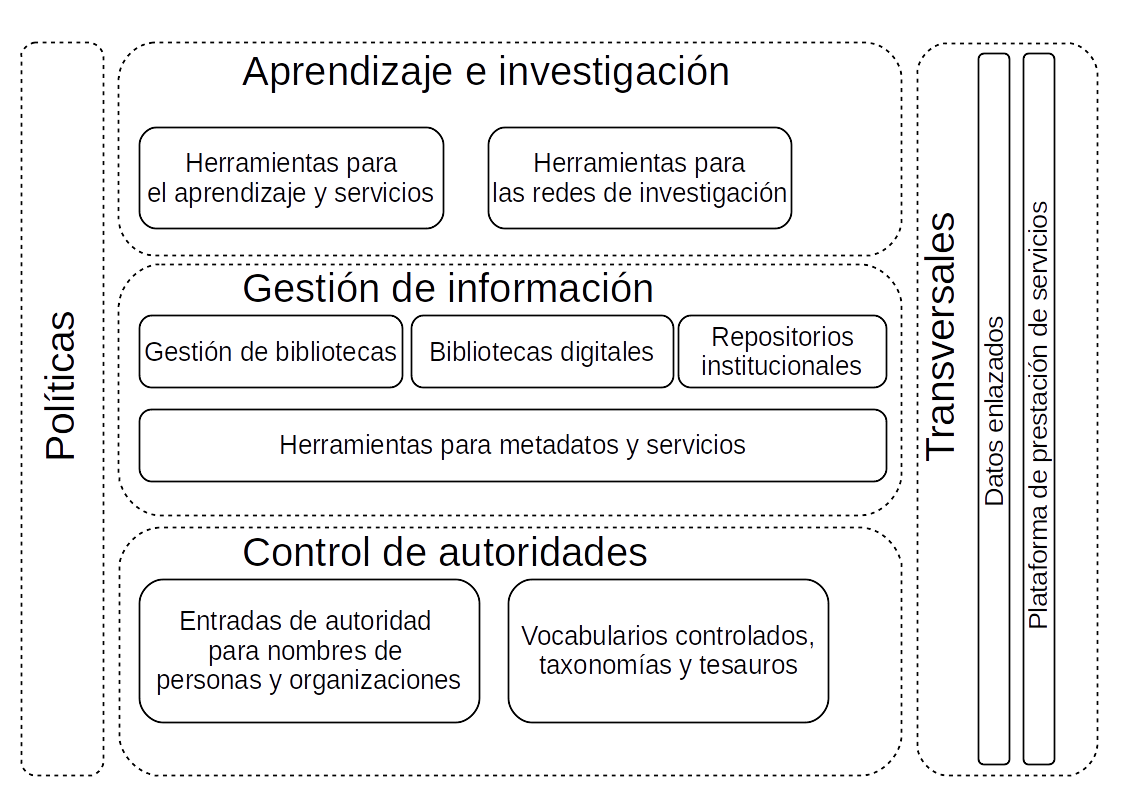
\includegraphics[width=0.5\textwidth]{img/referenceModel.png}
\end{center}
\caption{Modelo de referencia del proyecto ELINF. Fuente: Informe de autoevaluación de la primera fase del proyecto ELINF.}
\label{fig: referenceModel}
\end{figure}

En la redacción de artículos científicos se pueden encontrar variaciones de los nombres de un mismo autor, un autor puede tener varios nombres en artículos diferentes y varios autores pueden compartir el mismo nombre. Esta ambigüedad afecta el rendimiento de la recuperación de los documentos, la integración a nivel de bases de datos y puede causar atribuciones de autorías indebidas al aparecer los recursos descritos en los catálogos bajo un autor incorrecto \citep{Han2005}. En las bibliotecas, museos o en archivos un catálogo es un conjunto de datos organizados que describen los recursos de información gestionados por la institución \citep{InternationalFederationofLibraryAssociationsandInstitutions2009}, mientras que las personas encargadas de formar estos catálogos se denominan catalogadores \citep{RealAcademiaEspanola2014}. Durante al menos siglo y medio los catalogadores han documentado sus decisiones acerca de cómo la forma autorizada del nombre de una persona debería ser representada en sus catálogos \citep{Tillett2009}, sin embargo, según \cite{Carrasco2016} algunos tipos de inconsistencias que se encuentran a menudo en los nombres registrados en los catálogos son:

\begin{itemize}
\item Variantes del mismo nombre.
\item Permutaciones del nombre.
\item Errores tipográficos.
\item Eliminación de palabras vacías.
\item Eliminación de diacríticos.
\end{itemize}

Con la finalidad de evitar inconsistencias en los catálogos se realiza el control de autoridades, el cual es uno de los pilares del modelo de referencia del proyecto ELINF. El control de autoridades es el proceso de seleccionar una forma de un nombre y almacenarla, así como sus variantes y las fuentes de datos utilizadas en el proceso \citep{Sandberg2016}. Según \cite{Carrasco2016} este procedimiento sirve para dos propósitos fundamentales:

\begin{itemize}
\item Distinguir creadores que han publicado bajo el mismo nombre por medio de la adición de títulos y otras palabras asociadas con el nombre o incluyendo información sobre las fechas de nacimiento, muerte y actividad del mismo.
\item Identificar variantes del nombre o formas alternativas de escribirlo.
\end{itemize}

En el trabajo de las bibliotecas se ha estado lidiando con la identificación y desambiguación de los nombres de los creadores de los recursos de información desde los comienzos de la catalogación \citep{Harper2007}. Las diferentes formas utilizadas por el mismo creador en varias publicaciones y otros tipos de recursos siempre han acarreado cierto nivel de dificultad para agrupar sus creaciones \citep{Harper2007}.

Los catalogadores han creado registros para el control de autoridades durante décadas, resultando en grandes bases de datos con millones de registros como el ``Fichero de Nombres de Autoridades de la Biblioteca del Congreso'' (``Library of Congress Name Authority File'' - LC/NAF, por sus siglas de acuerdo al término en idioma inglés) \citep{Sandberg2016}.

Los ``Requerimientos Funcionales para Datos de Autoridad'' (``Functional Requirements for Authority Data'' – FRAD, por sus siglas de acuerdo al término en idioma inglés), elaborados en 2008 por la ``Federación Internacional de Asociaciones Bibliotecarias e Instituciones'' (``International Federation of Library Associations'' - IFLA, por sus siglas de acuerdo al término en idioma inglés), son un modelo entidad-relación enfocado en los datos de autoridad. Los FRAD enmarcan el control de autoridades en términos de entidades y relaciones entre personas y sus nombres; personas y sus obras, manifestaciones, expresiones y elementos \citep{InternationalFederationofLibraryAssociationsandInstitutions2009,Sandberg2016}.

El modelo que proponen los FRAD ha sido adoptado por las normas denominadas ``Recurso, Descripción y Acceso'' (``Resource, Description and Access''- RDA, por sus siglas de acuerdo al término en idioma inglés), que constituyen el código actual de control de autoridades \citep{Sandberg2016}.

Iniciativas existentes en la Web contribuyen a proveer mejores mecanismos para identificar a las personas que tienen un rol con respecto a recursos de información \citep{Harper2007}. ``Amigo de un amigo'' (``Friend of a friend'' - FOAF, por sus siglas de acuerdo al término en idioma inglés) es un proyecto que pretende crear una Web de páginas legibles por computadoras describiendo personas, sus vínculos y las cosas que crean y hacen. Encontrar formas de integrar este tipo de iniciativas con los mecanismos existentes en las bibliotecas para el control de autoridades puede contribuir a la inclusión de los catálogos bibliotecarios entre las herramientas disponibles en la Web. Adicionalmente, la disponibilidad de datos bibliotecarios de autoridad en formatos cada vez más compatibles con la Web, tiene el potencial para influenciar de manera positiva la organización de un amplio espectro de contenido disponible en la Web hoy día \citep{Harper2007}.

El ``Fichero Internacional Virtual de Autoridades'' (``Virtual International Authority File'' - VIAF, por sus siglas de acuerdo al término en idioma inglés) combina varios ficheros de nombres de autoridades en un solo servicio de nombres de autoridad. Para lograr esto, VIAF vincula los ficheros de autoridades de varias bibliotecas nacionales y agrupa todos los registros de autoridad para una entidad determinada en un ``súper registro de autoridad'' que unifica los diferentes nombres de dicha entidad \citep{OCLCOnlineComputerLibraryCenterInc.2014}.

Otra iniciativa ejecutada con el fin de contribuir al control de autoridades es el ``Identificador Internacional Estandarizado de Nombres'' (``International Standard Name Identifier'' - ISNI, por sus siglas de acuerdo al término en idioma inglés). ISNI es el número estándar global certificado para identificar a los contribuidores de trabajos creativos y a aquellos involucrados en su distribución como investigadores, inventores, escritores, artistas, creadores visuales, actores, productores entre otros \citep{ISNIInternationalStandardNameIdentifier2017}.

La misión de la Autoridad Internacional del ISNI (``ISNI International Authority'' - ISNI-IA, por sus siglas de acuerdo al término en idioma inglés) es asignarles a los nombres públicos de autores de recursos de información un número identificativo persistente con el objetivo de resolver el problema de la ambigüedad en la búsqueda y recuperación de la información respectiva a nombres de creadores de recursos de información \citep{ISNIInternationalStandardNameIdentifier2017}. Similares a esta iniciativa son las formas utilizadas por el Identificador Abierto de Investigador y Colaborador (``Open Researcher and Contributor ID'' - ORCID, por sus siglas de acuerdo al término en idioma inglés) \citep{ORCID2017} y el identificador de SCOPUS \citep{Elsevier2016}.

Con el objetivo de almacenar los datos con vistas a su posterior procesamiento y recuperación, variadas son las estructuras empleadas para realizar de forma eficiente esta tarea \citep{Gutierrez2011,Vavliakis2013,Lacasta2013}. Las bases de datos relacionales han sido empleadas durante varias décadas para estructurar los datos y recuperarlos de forma eficiente \citep{maier1983theory,Shanmugasundaram1999,Ilyas2004,Spanos2012}. En los últimos años la utilización de bases de datos ``No-SQL'' ha ganado popularidad con el objetivo de almacenar datos en forma de documentos \citep{Pokorny2013,Moniruzzaman2013}. La utilización del modelo de datos ``Marco de trabajo para la descripción de recursos'' (``Resource Description Framework'' - RDF, por sus siglas de acuerdo al término en idioma inglés) ha contribuido a aportar semántica a los datos almacenados, proveyendo un valor añadido a la información \citep{Berners-Lee2001,Konstantinou2014,Sule2016}.

En Cuba en el momento en que se realiza la presente investigación no existe un registro central para el control de autoridades, las instituciones realizan este proceso de forma aislada, provocando redundancia en el trabajo. De igual manera, no se reutilizan los registros de autoridades que comparten instituciones extranjeras. Esta situación dificulta la localización de la producción intelectual generada y/o almacenada en la Isla, a la vez que dificulta compartir las entradas de autoridad pertenecientes a autores cubanos con el resto del mundo.

La integración de fuentes de datos es el problema de interconectar y acceder a fuentes heterogéneas de datos \citep{Nachouki2011}. En la medida en que las organizaciones han evolucionado este problema se ha convertido en un importante campo de investigación tanto para la academia como para la industria \citep{Nachouki2011}. Aunque la dependencia conceptual es casi universal en el diseño de sistemas de información, también produce una gama de consecuencias negativas incluyendo la inflexibilidad de los sistemas, la heterogenidad en las formas de almacenar los datos, así como aumentos en los costos de mantenimiento \citep{McGinnes2015}. La heterogeneidad entre dos o más sistemas de bases de datos ocurre cuando estas utilizan diferente infraestructura de software o hardware, siguen diferentes convenciones sintácticas y modelos de representación o cuando interpretan de manera diferente datos similares \citep{Spanos2012}.

Con el propósito de contribuir a la solución de este problema en el pasado se propuso la creación de una base de datos federada (``Federated database'' - FDB, por sus siglas de acuerdo al término en idioma inglés) \citep{Sheth1990}. En arquitecturas de integración de bases de datos típicas, uno o más modelos conceptuales se utilizan para describir los contenidos de cada fuente de datos, las consultas se plantean en concordancia con un esquema conceptual global y para cada fuente de datos, una envoltura (``wrapper'', término utilizado en idioma inglés) es responsable de re-formular la consulta y recuperar los datos apropiados \citep{Spanos2012,Franke2014,ElKadiri2015}.

Un enfoque para la integración de datos empresariales provenientes de fuentes heterogéneas de datos y descentralizadas es la mediación semántica. Este enfoque por una parte elimina la necesidad de un repositorio central de datos o un esquema federado para todos los datos y, por otra parte, introduce una capa semántica encima de las descripciones de estructuras de datos sintácticas existentes para evitar los conflictos semánticos en la integración \citep{ElKadiri2015}. 

Con el advenimiento de la Web, la gestión de datos se enfocó en la variedad de información disponible en este nuevo medio. \cite{Janev2011} plantean que las tecnologías semánticas se utilizan en su mayoría para la integración de datos y para mejorar las búsquedas. Según \citep{Hoang2014}, la integración de datos guiada por ontologías representa una solución flexible, sostenible y extensible. Un paradigma reciente que combina la posibilidad de utilizar razonamiento sobre el conocimiento de un dominio codificado en una ontología, con un mecanismo que permite el uso de la misma ontología para un acceso integrado de alto nivel a las fuentes de datos es el Acceso e Integración de Datos Basado en Ontologías (``Ontology-Based Data Access and Integration'' - OBDA/OBDI, por sus siglas de acuerdo al término en idioma inglés) \citep{Calvanese2016,Calvanese2017}.

Teniendo en cuenta la heterogeneidad estructural de las fuentes de datos disponibles actualmente para realizar el control de autoridades en el proyecto ELINF se establece como \textbf{problema de investigación} el siguiente: ¿Cómo integrar los datos relativos al control de autoridades almacenados de forma heterogénea en las fuentes de datos utilizadas por el proyecto ELINF?

El problema de investigación se enmarca en el \textbf{objeto de estudio} la integración de datos almacenados de forma heterogénea y como \textbf{campo de acción} el método para integrar datos relativos al control de autoridades en el proyecto ELINF.

Esta investigación se propone como \textbf{objetivo general} desarrollar un método con componentes semánticos que permita la integración en una aplicación informática de datos relativos al control de autoridades, almacenados de forma heterogénea en las fuentes de datos utilizadas por el proyecto ELINF. Como \textbf{objetivos específicos} se definen los siguientes:

\begin{enumerate}
\item Identificar los referentes teóricos que soportan la integración semántica de datos en aplicaciones informáticas.
\item Desarrollar un método con componentes semánticos que permita integrar en una aplicación informática datos almacenados de forma heterogénea.
\item Evaluar el método desarrollado mediante un caso de estudio con datos reales relativos al control de autoridades almacenados de forma heterogénea.
\end{enumerate}

Se plantea como \textbf{hipótesis de la investigación} que, si se desarrolla un método con componentes semánticos para la integración de datos almacenados de forma heterogénea, será posible integrar los datos relativos al control de autoridades almacenados en las fuentes de datos utilizadas por el proyecto ELINF.

A partir de la hipótesis se identifica como variable independiente el \textbf{método con componentes semánticos} el cual se define como el conjunto de actividades \citep{Offermann2010} que permitirá conducir el proceso de descripción e integración de datos almacenados de forma heterogénea. Como variable dependiente se identifica la \textbf{integración de los datos relativos al control de autoridades} almacenados en las fuentes de datos utilizadas por el proyecto ELINF, definiéndose esta como la capacidad de mostrar en una vista conceptualmente homogénea datos de autoridades almacenados en fuentes heterogéneas de datos.


\begin{table}
\centering
\begin{tabular}{c|c|c}
\hline 
Variable & Dimensión & Indicadores \\ 
\hline 
Método con componentes semánticos & Etapas que lo componen & Artefactos generados \\ 
\hline 
Integración de los datos  & Fuentes integradas & Estructura de la fuente \\
relativos al control de autoridades & &  \\ 
 \hline
\end{tabular} 
\label{tabla:operacionalizacion}
\caption{Operacionalización de las variables de la investigación}
\end{table}


Durante toda la investigación se utilizará el método analítico - sintético, el mismo permitirá descomponer las problemáticas que se presenten en sus componentes y relaciones. La síntesis permitirá descubrir las relaciones esenciales existentes entre los componentes de las problemáticas contribuyendo a la sistematización del conocimiento. 

El método inductivo - deductivo posee especial relevancia en la formulación de la hipótesis y en la elaboración de conclusiones lógicas. Por medio del método histórico - lógico será posible representar los elementos del estado del arte relevantes a la temática en un orden cronológico que permita comprender la evolución de la misma.

El método hipotético - deductivo de conjunto con el inductivo - deductivo permitirá arribar a conclusiones particulares a partir de la hipótesis, que luego serán validadas experimentalmente. Esto posibilitará reafirmar la validez de la hipótesis de la investigación.

Por medio de la modelación será posible generar componentes relevantes para la aplicación del método propuesto, estando estrechamente relacionado con el método analítico - sintético y el método sistémico.

El documento de tesis está estructurado en tres capítulos, conclusiones y recomendaciones. A continuación, se brinda una breve descripción de cada uno de los capítulos.

El capítulo 1 aborda los principales referentes teóricos que soportan la integración semántica de datos, en él se refiere la evolución histórica del control de autoridades, se exponen los principales elementos de la Web Semántica y se relatan elementos de la integración de datos que son tomados en consideración para el desarrollo de la investigación.

En el capítulo 2 se identifica el paradigma utilizado en el desarrollo del método propuesto, se realiza la definición del método OntoIntegra a la vez que se describen cada uno de sus componentes. Se detalla el proceso de desarrollo de la ontología creada según la metodología seleccionada, generando cada uno de los artefactos definidos.

El capítulo 3 relata la selección de la estrategia de evaluación, la preparación del caso de estudio, su diseño con cada una de las etapas que lo componen. Se realiza un análisis de los datos recolectados que permite comprobar la validez de la hipótesis formulada para conducir la investigación.
    \newpage
   
    \renewcommand{\chaptermark}[1]{\markright{\hfill \chaptername \space \thechapter.\ #1.}}
    \rhead{\chaptermark}
    \chapter{\large Fundamentación teórica}

\pagestyle{fancy}
\lhead{}
\chead{}
\rhead{Capítulo 1: Fundamentación teórica}
\lfoot{}
\cfoot{}
\rfoot{\thepage}
\renewcommand{\headrulewidth}{0.4pt}
%\renewcommand{\footrulewidth}{0.4pt}
 \vspace{-1cm}

%\lettrine[lines=2, lraise=0, nindent=0em, slope=-.5em]
\section{Introducción}
En este capítulo se abordan los principales referentes teóricos que soportan la integración semántica de datos. Primeramente se refiere la evolución histórica del control de autoridades con el objetivo de contextualizar el área de aplicación del método que se propone en el presente trabajo. En la sección 1.3 se aborda la Web Semántica describiendo sus principales elementos, los cuales intervienen en la aplicación del método propuesto. Posteriormente se relatan elementos de la integración de datos que se toman en consideración para el desarrollo de la investigación.
\section{Control de autoridades}
El control de autoridades es un problema global que afecta a organizaciones de diversos tipos \citep{Leiva-Mederos2013}. La comunidad bibliotecaria durante largo tiempo ha sido consciente de la necesidad del control de autoridades \citep{Harper2007,Tillett2009,Leiva-Mederos2013,Carrasco2016}. La necesidad de almacenar uniformemente la información correspondiente a cada autor incluido en un catálogo es abordada en el trabajo y la investigación de varias organizaciones internacionales \citep{Leiva-Mederos2013}. Una panorámica breve del desarrollo en el control de autoridades incluiría los siguientes elementos:

\begin{itemize}
\item Se hace explícita la necesidad del control de autoridades y surge la ``Cooperación en Nombres de Autoridades'' (``Name Authority Cooperative'' - NACO, por sus siglas de acuerdo al término en idioma inglés) en la ``Biblioteca del Congreso'' (``Library of Congress'' - LOC, por sus siglas de acuerdo al término en idioma inglés) de los Estados Unidos de América \citep{Leiva-Mederos2013}. En Asia se establece el ``Nombre de Autoridad de Hong Kong Chino'' (``Hong Kong Chinese Authority Name'' - HKCAN, por sus siglas de acuerdo al término en idioma inglés). Esto significó el reconocimiento de la problemática por dos organizaciones internacionales a partir de los elementos enunciados en el siglo XIX por \cite{cutter1889rules}.

\item \cite{lubetzky1969principles} mejoran la búsqueda y recuperación de trabajos en catálogos bibliográficos.

\item \cite{bregzis1982syndetic} crea el ``Número Internacional Estandarizado de Datos de Autoridad'' (``International Standard Authority Data Number'' - ISADN, por sus siglas de acuerdo al término en idioma inglés) con el fin de vencer las dificultades al recuperar registros bibliográficos con trabajos relativos a un autor en específico y trabajos almacenados bajo un título uniforme.

\item La LOC crea el ``Fichero de autoridad NACO de la LOC'' (``Library of Congress/NACO Authority File'' - LC/NAF, por sus siglas de acuerdo al término en idioma inglés) \citep{Sandberg2016}.

\item La ``Federación Internacional de Asociaciones de Bibliotecarios y Bibliotecas'' (``International Federation of Library Asociations and Institutions'' - IFLA, por sus siglas de acuerdo al término en idioma inglés) crea los FRAD \citep{InternationalFederationofLibraryAssociationsandInstitutions2009}.

\item El ``Centro Bibliotecario Computarizado En Línea'' (``Online Computer Library Center'' - OCLC, por sus siglas de acuerdo al término en idioma inglés) crea el VIAF \citep{OCLCOnlineComputerLibraryCenterInc.2014}.
\end{itemize}

La necesidad de crear registros de autoridad de alta calidad ha impulsado la creación de herramientas como AUTHORIS \citep{Leiva-Mederos2013}. AUTHORIS aspira a facilitar el procesamiento de datos de autoridad en una manera estandarizada siguiendo los principios de los Datos Enlazados Abiertos \citep{Berners-Lee2006}.

\section{Web Semántica}
La Web 2.0 se basa en un conjunto de tecnologías y estándares definidos por el ``Consorcio World Wide Web'' (``World Wide Web Consortium'' - W3C, por sus siglas de acuerdo al término en idioma inglés) entre los que se encuentra el ``Protocolo de Transferencia de Hipertextos'' (``Hypertext Transfer Protocol'' - HTTP, por sus siglas de acuerdo al término en idioma inglés), los ``Identificadores de Recursos Universales'' (``Universal Resource Identifier'' - URI, por sus siglas de acuerdo al término en idioma inglés) y el ``Lenguaje de Marcado de Hipertextos'' (``Hypertext Markup Language'' - HTML, por sus siglas de acuerdo al término en idioma inglés) para la representación de contenidos \citep{Masinter2005}. Este último carece de un mecanismo para expresar el significado de los contenidos publicados, imposibilitando a las computadoras procesar los mismos automáticamente \citep{Hidalgo-Delgado2015}.

El significado del término Web Semántica es definido por \cite{Berners-Lee2001} en un artículo donde expresa: \textit{La Web Semántica no es una Web aparte, sino una extensión de la existente en la que la información posee significado formalmente definido, facilitando que las computadoras y los humanos trabajen cooperativamente}. 

\subsection{Marco de Trabajo para la Descripción de Recursos}

Con el objetivo de proporcionar un formato único procesable por computadoras para la representación y descripción de los datos en la Web Semántica, la W3C define el ``Marco de Trabajo para la Descripción de Recursos'' (``Resource Description Framework'' - RDF, por sus siglas de acuerdo al término en idioma inglés), el cual consiste en un modelo de datos simple y totalmente compatible con la Web 2.0 \citep{motik2009bridging,Heath2011}.

Un documento RDF consiste en un conjunto de tripletas de la forma sujeto-predicado-objeto (Figura \ref{fig:Modelo de datos basado en grafo del estándar RDF}) de manera que los datos puedan ser representados en un grafo dirigido donde la primera y la tercera componente corresponde a los nodos del grafo y la segunda componente (predicado) actúa como enlace (arco) entre dichos nodos. Al grafo dirigido descrito anteriormente se le conoce como Grafo RDF y utiliza las ontologías para la descripción formal de los datos en términos de clases y propiedades \citep{Klyne2004}.

\begin{figure}
	\centering
	  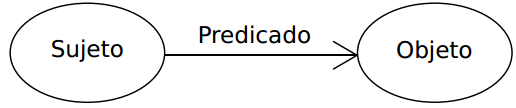
\includegraphics[width=12cm]{img/graficoRDF.png}
	\caption{Modelo de datos basado en grafo del estándar RDF}
	\label{fig:Modelo de datos basado en grafo del estándar RDF}
\end{figure}

\subsection{Ontologías}

La evolución del RDF en el ``Lenguaje de Ontologías Web'' (``Web Ontology Language'' - OWL, por sus siglas de acuerdo al término en idioma inglés) permite una descripción semántica más rica basada en Lógica Descriptiva \citep{Horrocks}. El OWL ha sido utilizado en varios escenarios específicos para la construcción de modelos de datos flexibles \citep{Agus,Munir,Franke2014,Sule2016}. 

El término ontología es utilizado con diferentes significados en diferentes comunidades. Su origen se encuentra en la filosofía y son utilizadas para estudiar la naturaleza del ser y su existencia \citep{Gruber1993,Gomez-Perez2004}. En computación una definición ampliamente aceptada fue formulada por \cite{Gruber1993} el cual afirma que \textit{una ontología es una especificación explícita de una conceptualización}. Años más tarde \cite{Studer1998} se basan en este concepto y lo extienden, afirmando que \textit{una ontología es una especificación formal y explícita de una conceptualización compartida}. Según \cite{Studer1998} una ontología:

\begin{itemize}
\item Es explícita porque define los conceptos, propiedades, relaciones, funciones, axiomas y restricciones que la componen.
\item Es formal porque es legible e interpretable por computadoras.
\item Es una conceptualización porque es un modelo abstracto y una vista simplificada de los elementos reales que representa.
\item Es compartida porque se ha arribado previamente a un consenso sobre la información y es aceptada por un grupo de expertos.
\end{itemize}

\cite{Staab2009} afirman que existen cuatro tipos diferentes de ontologías a diferentes niveles de granularidad. En un nivel superior se encuentran las ontologías fundacionales, las cuales capturan conceptos generales independientes de un dominio específico. En un segundo nivel de abstracción se encuentran las ontologías de dominio, las cuales modelan conceptos y relaciones que son relevantes para un dominio específico. En estas ontologías se suelen utilizar los términos de la ontologías fundacionales.

Otro tipo de ontología son las ontologías de tareas, las cuales describen conceptos de una tarea en específico. A un nivel más bajo de abstracción se encuentran las ontologías de aplicaciones. Estas combinan ontologías de dominio y ontologías de tareas extendiéndolas con nuevos conceptos y relaciones más específicos \citep{Staab2009}.

\cite{Gruber1993} y \cite{Gomez-Perez2004} proponen que las ontologías se modelen utilizando cinco tipos de componentes: clases, relaciones, funciones, instancias y axiomas formales. Las \textbf{clases} representan conceptos que pueden ser abstractos o no. Las clases de una ontología comúnmente se organizan en taxonomías a través de las cuales se pueden aplicar mecanismos de herencia.

Las \textbf{relaciones} representan tipos de asociaciones entre conceptos del dominio. Formalmente se pueden definir como cualquier subconjunto del producto de $n$ conjuntos, esto es $R \subset C_1 \,\times \,C_2 \,\times \ldots \times \,C_n$. Las ontologías con frecuencia poseen relaciones binarias, donde el primer argumento es conocido como el dominio y el segundo como el rango \citep{Gomez-Perez2004}.

Las \textbf{funciones} son un caso especial de relaciones donde el $n$-ésimo elemento de la relación es único para los $n-1$ elementos precedentes, es decir, $F: C_1 \,\times \,C_2 \,\times \ldots \times \,C_{n-1} \rightarrow C_n$ \citep{Gomez-Perez2004}.

Las \textbf{instancias} se utilizan para representar los individuos en una ontología \citep{Gomez-Perez2004}.

Según \cite{Gruber1993} los axiomas formales sirven para modelar sentencias que siempre son verdaderas. Normalmente se usan para representar conocimiento que no puede ser definido formalmente por otros componentes. Además, los axiomas formales se usan para verificar la consistencia de la ontología en sí misma o la consistencia del conocimiento almacenado en una base de conocimiento \citep{Gomez-Perez2004}. 

\subsection{Metodologías para el desarrollo de ontologías}

La Ingeniería Ontológica es la disciplina que estudia los principios, métodos y herramientas para crear y mantener ontologías. Una metodología de Ingeniería Ontológica proporciona el aspecto metodológico del desarrollo de ontologías. Con el objetivo de asistir a los ingenieros ontológicos y a los expertos de dominio en la construcción de ontologías se han desarrollado varias metodologías para la Ingeniería Ontológica \citep{Iqbal2013}.

Un análisis en profundidad de las principales metodologías para el desarrollo de ontologías es realizado por \cite{Iqbal2013}, estos autores proponen ocho criterios para la comparación de metodologías que se detallan a continuación.

\textbf{Criterio 1. Tipo de desarrollo}

La literatura revela que las metodologías para el desarrollo de ontologías pueden dividirse en tres categorías fundamentales: modelos basados en etapas, modelos de prototipos evolutivos y guías; dependiendo del tipo de modelo de desarrollo que siguen. Los diferentes enfoques tienen sus aspectos positivos y negativos. Las metodologías basadas en etapas pueden ser factibles en escenarios donde el propósito y los requerimientos están claramente definidos. Por el contrario, los prototipos evolutivos pueden ser la mejor elección cuando los requerimientos no están claramente definidos desde el inicio y es necesario refinar la ontología con el paso del tiempo. Las guías mayormente se enfocan en hacer sugerencias útiles, recomendar reglas y técnicas con el objetivo de tomar mejores decisiones en lugar de enfocarse en el modelo de desarrollo en sí.

\textbf{Criterio 2. Soporte para la construcción colaborativa}

Las ontologías pueden construirse tanto de forma aislada como colaborativamente. El soporte para la construcción colaborativa permite a diferentes miembros del equipo de desarrollo de ontologías trabajar en una misma ontología a la vez. Los miembros del equipo de desarrollo pueden estar dispersos geográficamente sin afectar la eficiencia del proyecto. 

\textbf{Criterio 3. Soporte para re-utilización}

El desarrollo de ontologías es una tarea costosa en tiempo y esfuerzo. Con el fin de economizar estos factores la noción de ontologías re-utilizables ha cobrado fuerzas a lo largo del tiempo. Las metodologías que soportan la re-utilización les permiten a los equipos de desarrollo de ontologías hacer uso de ontoloogías ya existentes reduciendo el tiempo y esfuerzo empleado en el desarrollo. El ahorro del tiempo les permite a los ingenieros enfocarse en los defectos presentes en las ontologías existentes, mejorando su calidad. 

\textbf{Criterio 4. Soporte para interoperabilidad}

Las ontologías de dominio que se desarrollen utilizando metodologías que soporten la interoperabilidad, proveerán a los sistemas que las usen de los mismos conceptos de alto nivel, por lo que les será más fácil comunicarse y compartir la información que gestionan entre sí.

\textbf{Critero 5. Grado de dependencia de la aplicación}

Diferentes metodologías durante el proceso de desarrollo pueden adoptar diferentes enfoques en cuanto a la dependencia de una aplicación. Una metodología puede optar por uno de tres escenarios: dependiente de la aplicación (la ontología se desarrolla enfocada en la base de conocimiento para una aplicación específica), semi-independiente de la aplicación (la ontología se desarrolla teniendo en cuenta posibles escenarios de aplicación durante la etapa de especificación) e independiente de la aplicación (la ontología se desarrolla sin enfocarse en un sistema en particular).

\textbf{Criterio 6. Recomendación del ciclo de vida}

El ciclo de vida de una ontología identifica el conjunto de etapas por las que pasa una ontología durante su vida. Varias metodologías no recomiendan claramente un ciclo de vida.

\textbf{Criterio 7. Estrategias para la identificación de conceptos}

La identificación de los conceptos candidatos para la inclusión en la ontología es indudablemente un proceso crucial en el desarrollo de la misma. Existen técnicas para la identificación de conceptos, algunas de ellas utilizan un enfoque abajo - arriba, mientras que otras emplean un enfoque arriba - abajo y unas terceras el enfoque que siguen es del centro hacia afuera.

\textbf{Criterio 8. Nivel de detalle de la metodología}

Cada metodología comprende algunas actividades y técnicas para soportar el desarrollo de ontologías. El análisis de la literatura ha revelado la existencia de metodologías que no proveen suficientes detalles para el empleo de sus actividades y técnicas. Para propósitos de análisis, este trabajo clasificará las metodologías en tres grupos de acuerdo a este criterio: suficientes detalles, algunos detalles e insuficientes detalles. Las metodologías que no brindan detalles o estos son muy vagos se clasificarán como de insuficientes detalles. Por otra parte, las metodologías que no cubren completamente los detalles pero al menos proporcionan algunos detalles sobre sus actividades y técnicas se clasificarán como algunos detalles. Asimismo, las metodologías clasificadas como suficientes detalles proveen un razonable nivel de detalles sobre las actividades y técnicas que emplean, permitiendo al lector comprenderlas claramente. 

Una clasificación de las metodologías analizadas de acuerdo a los criterios anteriormente expuestos se brinda en el trabajo de \cite{Iqbal2013}. Posterior al análisis de diferentes metodologías para el desarrollo de ontologías se decidió utilizar para el presente trabajo METHONTOLOGY ya que recomienda un ciclo de vida, es reutilizable y provee suficientes detalles sobre las técnicas y actividades empleadas en ella.

\subsection{Datos Enlazados Abiertos}
Los Datos Enlazados Abiertos son un conjunto de principios y buenas prácticas para la publicación de datos en la Web. Estos datos pueden estar dispersos geográficamente y pertenecer a una o varias organizaciones. En este sentido \cite{Berners-Lee2006} propone cuatro principios:

\begin{enumerate}
\item Utilizar URIs como nombres para las cosas.

\item Utilizar URIs HTTP para que las personas puedan buscar esos nombres.

\item Cuando alguien busca una URI, proveer información útil por medio de los estándares.

\item Incluir vínculos a otras URIs para que se puedan descubrir más cosas.
\end{enumerate}

El primer principio propone el uso de URIs para identificar no solo documentos web y contenido digital, sino que sirva además para referenciar a objetos del mundo real y conceptos abstractos. El segundo principio propone el uso de URIs basadas en el protocolo HTTP para identificar objetos y conceptos abstractos, posibilitando que estas URIs estén desreferenciadas sobre dicho protocolo y en cambio proporcionen una descripción del objeto o concepto identificado. El tercer principio propone el uso del modelo de datos RDF para publicar datos estructurados en la Web. El cuarto principio propone el uso de enlaces para enlazar no solo documentos web, sino cualquier tipo de recurso \citep{Hidalgo-Delgado2015}.

\section{Integración de datos}
Actualmente la existencia, competitividad y rentabilidad de diversas compañías depende de los flujos de datos. Sin embargo, la variedad de fuentes, tipos y volúmenes de datos ha vuelto más complejo el proceso de encontrarlos \citep{AloomaInc.2017}. La integración de datos se refiere a las técnicas involucradas en combinar los datos almacenados en diferentes ubicaciones en una vista común integrada \citep{Michel2017}. La disponibilidad de recursos de información heterogéneos y distribuidos ha conducido a considerar aproximaciones para la integración de datos en los que fuentes de datos independientes puedan participar en federaciones virtuales de datos. Mientras que los almacenes de datos son repositorios rígidos controlados por las premisas de una sola compañía, las nuevas necesidades de información deben acomodarse a la adición oportuna de nuevas fuentes de datos provenientes de instituciones independientes.

Por otra parte, la semántica de los datos almacenados en ocasiones no es descrita por los esquemas de bases de datos. Hasta cierto punto la semántica implícita de los datos se puede inferir a partir de las restricciones de integridad o patrones de diseño de bases de datos comunes, pero la semántica adicional se encuentra codificada en las aplicaciones que consumen las fuentes de datos. Además, frecuentemente los esquemas de bases de datos se optimizan por cuestiones de rendimiento, resultando en una mezcla de la semántica de los datos con aspectos técnicos. Por estas razones, los métodos utilizados para la integración de datos en la Web deben poseer la capacidad de capturar y compartir conceptualizaciones formales comunes en una manera explícita 
procesable por computadoras. Esto convencionalmente se logra por medio de la utilización de vocabularios controlados, tesauros y ontologías.

\subsection{Principios para la integración de datos}
Convencionalmente, un sistema para la integración de datos $\Psi$ se denota por la tupla $<\Gamma , \Upsilon , \Sigma>$ donde:

\begin{itemize}
\item $\Gamma$ es el esquema global utilizado para representar la vista unificada.
\item $\Upsilon$ son las fuentes de datos representadas por el conjunto de esquemas locales $\upsilon_1 , \cdots , \upsilon_n$.
\item $\Sigma$ especifica las correspondencias entre los conceptos de los esquemas locales y los conceptos del esquema global.
\end{itemize}

Dependiendo de los lenguajes de modelado utilizados para definir los esquemas locales y globales, los conceptos pueden ser clases de una ontología, tablas de una base de datos, objetos, entre otros.

Un sistema para la integración de datos responde a consultas formuladas en términos del esquema global $\Gamma$ reformulándolas en las consultas correspondientes sobre las fuentes de datos $\upsilon_1 , \cdots , \upsilon_n$ por medio de la información almacenada en $\Sigma$. Con respecto a la forma en que se expresan los mapeos se han propuesto dos enfoques principales: el enfoque ``Global-como-Vista'' (``Global-as-View'' - GAV, por sus siglas de acuerdo al término en idioma inglés), en el que el esquema global se expresa en términos de consultas (o vistas) sobre los esquemas locales; mientras que en el enfoque ``Local-como-Vista'' (``Local-as-View'' - LAV, por sus siglas de acuerdo al término en idioma inglés), los esquemas globales se expresan en términos de consultas (o vistas) sobre el esquema global. Estos enfoques han sido abundantemente descritos en la literatura \citep{Doan:2012:PDI:2401764,Lenzerini:2002:DIT:543613.543644}.

Variados son los sistemas propuestos para la integración de datos basados en RDF, unos en forma de motores de consultas federados sobre SPARQL \citep{Schwarte:2011:FOT:2063016.2063055,Gorlitz:2011:SSE:2887352.2887354,Corby:2012:KVI:2457524.2457672,macina2016sparql} y otros como fragmentos de Datos Enlazados \citep{VERBORGH2016184}. Sin embargo, los enfoques de estos sistemas no se pueden clasificar claramente como GAV o LAV porque sus objetivos son producir planes de consultas eficientes sobre fuentes de datos distribuidas que soportan SPARQL sin la mediación de un esquema.

\subsection{Acceso e Integración de Datos Basado en Ontologías}\label{Acceso e Integración de Datos Basado en Ontologías}
El ``Acceso a Datos Basado en Ontologías'' (``Ontology-based Data Access'' - OBDA, por sus siglas de acuerdo al término en idioma inglés) es un dominio de la Integración de Datos que propone la utilización de ontologías para crear una capa conceptual formal; en esta capa la ontología representa el dominio de los datos almacenados en la fuente de datos y el mapeo describe las relaciones entre la ontología y la fuente de datos \citep{Calvanese:2015:SOY:2991147.2991152,KHARLAMOV20173}. \cite{Tabares-Martin2016} definen formalmente un sistema OBDA como una tupla \( \Omega = <\tau,\sigma,\mu> \) donde:

\begin{itemize}
 	\item \(\tau\) es la parte terminológica de la ontología. Se consideran ontologías basadas en Lógica Descriptiva, por lo que $\tau$ es una TBox según la Lógica Descriptiva.
 	\item $\sigma$ es el conjunto de fuentes de datos.
 	\item $\mu$ es un conjunto de mapeos, cada uno de la forma $\Phi(x) \leftarrow \Xi(x)$ donde:
 	\begin{itemize}
 		\item[•] $\Phi(x)$ es una consulta sobre $\sigma$, retornando las tuplas de valor para $x$.
 		\item[•] $\Xi(x)$ es una consulta sobre $\tau$ cuyas variables libres provienen de $x$.
 	\end{itemize}
\end{itemize}

La ontología en el paradigma OBDA provee un punto de acceso único para un acceso a datos semántico destinado a los consumidores de datos, a la vez que permite exportar los datos de las fuentes integradas en un formato semántico o ejecutar consultas en términos de un modelo conceptual orientado al usuario que lo abstraen de los detalles a nivel de implementación que comúnmente se encuentran en los esquemas de bases de datos \citep{KHARLAMOV20173}. Por otra parte, los expertos en el dominio son capaces de expresar las necesidades de información en sus propios términos sin conocimiento previo sobre la forma en que están estructurados los datos en la fuente, a la vez que reciben las respuestas a sus consultas en los términos definidos en la ontología.

La ``Integración de Datos Basada en Ontologías'' (``Ontology-based Data Integration'' - OBDI, por sus siglas de acuerdo al término en idioma inglés) es un caso más general de OBDA en el cual las organizaciones gestionan de forma integrada diferentes fuentes de datos por medio del paradigma OBDA. La OBDI se ha utilizado en trabajos como los descritos por \cite{Calvanese2016,Daraio2016,Kharlamov:2016:OIS:2882903.2899385}

\section{Conclusiones del capítulo}
El objetivo que persigue este trabajo es desarrollar un método con componentes semánticos que permita la integración en una aplicación informática de datos relativos al control de autoridades almacenados de forma heterogénea. En este capítulo se abordó el control de autoridades realizando un análisis histórico de su desarrollo que permitió conocer su evolución e identificar los problemas actuales existentes en la temática. Posteriormente se analizaron diferentes elementos que forman parte de las tecnologías de la Web Semántica y que posibilitan describir semánticamente los datos almacenados en fuentes estructuralmente heterogéneas. Luego se examinaron principios para la integración de datos, haciendo énfasis en la integración semántica de datos.

Al realizar la revisión bibliográfica respectiva al estado del arte de la temática se evidenciaron diferentes aproximaciones que posibilitan la integración semántica de datos, siendo la Integración de Datos Basada en Ontologías una de las más promisorias. Sin embargo, a pesar de que se describen los elementos que intervienen en la OBDI, en la literatura revisada no se especifica un método para llevarla a cabo.









    \chapter{\large Método para la integración de datos basada en ontologías}


\pagestyle{fancy}
\lhead{}
\chead{}
\rhead{Capítulo 2: Método para la integración de datos basada en ontologías}
\lfoot{}
\cfoot{}
\rfoot{\thepage}
\renewcommand{\headrulewidth}{0.4pt}
%\renewcommand{\footrulewidth}{0.4pt}
 \vspace{-1cm}

\section{Paradigma utilizado en el desarrollo del método}
La investigación en la disciplina de sistemas de información (SI) se caracteriza por dos paradigmas: las ciencias del comportamiento y las ciencias del diseño \citep{Hevner:2004:DSI:2017212.2017217}. El primer paradigma persigue el desarrollo y verificación de teorías que expliquen o pronostiquen el comportamiento humano u organizacional. El paradigma de las ciencias del diseño tiene como fin la creación de innovaciones que definan ideas prácticas, capacidades tecnológicas y productos a través de los cuales puede lograrse el análisis, diseño, implementación, gestión y uso de sistemas de información de manera efectiva y eficiente \citep{Denning:1997:NSC:253671.253755}. Analizando la naturaleza del problema tratado en esta investigación y la relación entre su campo de acción (el mecanismo para integrar datos relativos al Control de Autoridades en la aplicación informática AUCTORITAS) y la disciplina de SI, el desarrollo de la solución se concibió y ejecutó bajo el paradigma de las ciencias del diseño.

Las ciencias del diseño crean y evalúan artefactos orientados a mejorar y entender el comportamiento de los sistemas de información, estos artefactos pueden ser constructos, modelos, métodos e instanciaciones \citep{March:1995:DNS:1700865.1700867}. Los constructos pertenecen al vocabulario conceptual de un dominio y son empleados por los modelos para representar una situación del mundo real en términos del diseño de un problema y su espacio de solución \citep{Simon:1996:SA:237774}. La búsqueda dentro de ese espacio de solución es guiada por métodos, los cuales pueden ser algoritmos matemáticos, descripciones textuales del proceso de búsqueda o combinaciones de ambas \citep{Hevner:2004:DSI:2017212.2017217}. Las instanciaciones demuestran la viabilidad de implementar los métodos y modelos, a la vez que facilitan la evaluación concreta del artefacto que representan.


    %\chapter{\large Evaluación de la propuesta}\label{Capítulo 3}

\pagestyle{fancy}
\lhead{}
\chead{}
\rhead{Capítulo 3: Evaluación de la propuesta}
\lfoot{}
\cfoot{}
\rfoot{\thepage}
\renewcommand{\headrulewidth}{0.4pt}
%\renewcommand{\footrulewidth}{0.4pt}
\vspace{-1cm}

\section{Introducción}
sdfsd

\section{Selección de la estrategia de evaluación}
Dependiendo del propósito de la evaluación y de las condiciones de la investigación empírica, existen tres grandes tipos de estrategias que pueden utilizarse: encuestas, casos de estudio y experimentos \citep{Wohlin2012}.

Una encuesta es un sistema para recolectar información sobre o acerca de personas que describen, comparan o explican su conocimiento, actitudes y comportamiento \citep{Wohlin2012}. Una encuesta no permite el control sobre la ejecución de la medición, por lo que no es posible manipular variables como en otros métodos de investigación \citep{Wohlin2012}.

Los casos de estudio en la ingeniería de software son investigaciones empíricas que se basan en múltiples fuentes de evidencia para investigar una instancia (o un pequeño número de ellas) de un fenómeno de ingeniería de software contemporáneo dentro de su contexto real, especialmente cuando el límite entre el fenómeno y el contexto no puede ser claramente definido \citep{Runeson:2012:CSR:2361717,Wohlin2012}. Constituyen una técnica donde factores clave que pueden incidir en la salida se identifican y se documenta la actividad \citep{stake1995art}. 

Los experimentos (o experimentos controlados) en la ingeniería de software son un tipo de investigación empírica que manipula un factor o variable de la configuración estudiada. Basado en la aleatoriedad se aplican diferentes tratamientos a diferentes sujetos, mientras se mantienen otras variables constantes y se miden los efectos en las variables de salida \citep{Wohlin2012}. Constituyen una investigación formal, rigorosa y controlada en la que los factores claves son identificados y manipulados, mientras que otros factores en el contexto se mantienen sin cambio. 

La diferencia entre casos de estudio y experimentos está determinada por el nivel de control del contexto \citep{Petersen:2009:CIS:1671248.1671293}. En un experimento diferentes situaciones son forzadas deliberadamente y el objetivo comúnmente es distinguir entre las dos situaciones. En un caso de estudio el contexto es controlado por el proyecto real analizado \citep{Wohlin2012}. Basados en los elementos expuestos, el autor de la presente investigación concluye que la realización de un caso de estudio constituye una estrategia viable para la evaluación de la misma. 

\section{Preparación del caso de estudio}
Según \cite{kitchenham1995case} para evitar el sesgo y asegurar la validez interna, es necesario crear una base sólida para evaluar los resultados de un caso de estudio. \cite{kitchenham1995case} proponen tres alternativas para preparar un estudio con el fin de facilitar esto:

\begin{itemize}
\item Una comparación de los resultados aplicando el método contra una línea base es una solución.
\item Un proyecto hermano puede ser seleccionado como línea base. El proyecto bajo estudio emplea el nuevo método mientras que el proyecto hermano usa los métodos anteriores. Ambos proyectos deben ser comparables.
\item Si el método se aplica a componentes del producto individuales, debe ser aplicado aleatoriamente a algunos componentes y a otros no.
\end{itemize}

Para el caso de estudio en cuestión se utilizarán las versiones 1.0 y 2.0 de la aplicación informática AUCTORITAS. La versión 1.0 de AUCTORITAS utiliza un acceso a datos incrustado en el código fuente de la aplicación y, para incorporar nuevas fuentes de datos, es necesario modificar su código fuente.

El acceso a datos de la versión 2.0 de AUCTORITAS se desarrolló empleando el método propuesto en la presente investigación. El mismo depende de la conceptualización definida en una ontología y es extensible por medio de la modificación de la T-Box de la ontología, sin necesidad de modificar el código fuente de la aplicación.

Según \cite{Wohlin2012}, la realización de un caso de estudio involucra cinco grandes pasos por los que transitar:

\begin{enumerate}
\item Diseño del caso de estudio: se definen los objetivos y se planifica el caso de estudio.
\item Preparación para la recolección de los datos: se definen los procedimientos y protocolos para la recolección de los datos.
\item Recolección de los datos: ejecución de la recolección de los datos en el caso estudiado.
\item Análisis de los datos recolectados.
\item Reporte del caso de estudio.
\end{enumerate}

\subsection{Diseño del caso de estudio}
El \textbf{objetivo} del presente caso de estudio es \textbf{medir el nivel de flexibilidad que aporta aplicar el método propuesto en el desarrollo del acceso a datos de la aplicación informática AUCTORITAS}. Se definen los siguientes umbrales para la variable flexibilidad:

\begin{itemize}
\item Flexibilidad baja: es necesario modificar el código fuente de la aplicación para adicionar nuevas fuentes de datos y estas deben ser estructuralmente homogéneas.
\item Flexibilidad media: es necesario modificar el código fuente de la aplicación para adicionar nuevas fuentes de datos pero estas pueden ser estructuralmente heterogéneas.
\item Flexibilidad alta: no es necesario modificar el código fuente de la aplicación para adicionar nuevas fuentes de datos y estas pueden ser estructuralmente heterogéneas.
\end{itemize}

El presente caso de estudio se centra en la escalabilidad en cuanto a fuentes de datos de la aplicación informática AUCTORITAS. Se asume como escalabilidad el concepto elaborado por \cite{duboc2006framework} que la define como la cualidad de las aplicaciones informáticas caracterizada por el impacto causal que poseen aspectos del entorno del sistema según estos son variados por encima de los rangos operacionales.

Las preguntas de investigación que conducirán el presente caso de estudio son:

\begin{enumerate}
\item ¿Qué fuentes de datos de las necesarias para el control de autoridades en el proyecto ELINF es posible integrar con el método propuesto?
\item ¿Qué nivel de flexibilidad aporta la aplicación del método propuesto en el acceso a datos de la aplicación informática AUCTORITAS?
\end{enumerate}

Para la recolección de los datos se utilizará el formato de la tabla \ref{tabla: recoleccion}.

\begin{table}
\centering
\begin{tabular}{c|c|c|c}
\hline 
Aplicación informática & Fuente de datos & Estructura & Modificación código fuente \\ 
\hline 
& & & \\
\hline
\end{tabular} 
\caption{Tabla para recolectar datos en el caso de estudio.}
\label{tabla: recoleccion}
\end{table}


    %\chapter{\large Implementación y prueba.}


\pagestyle{fancy}
\lhead{}
\chead{}
\rhead{Capítulo 4: Implementación y prueba}
\lfoot{}
\cfoot{}
\rfoot{\thepage}
\renewcommand{\headrulewidth}{0.4pt}
%\renewcommand{\footrulewidth}{0.4pt}
 \vspace{-1cm}

\begin{enumerate}
 \item[a] {\bf \lettrine[lines=2, lraise=0, nindent=0em, slope=-.5em]{I}{}mplementación.}
  \begin{itemize}
    \item Diagrama de despliegue.
    \begin{longtable}[c]{|l|}
      \hline
      \rowcolor{gray}
      \multicolumn{1}{|>{\columncolor{Light}}c|}{DIAGRAMA DE DESPLIEGUE}\\
      \hline
      \multicolumn{1}{|c|}{(1)}\\
      \hline
    \end{longtable}
    {\bf Leyenda}
    \begin{enumerate}
     \item Representación gráfica del diagrama.
    \end{enumerate}

  \item Diagrama de componentes.
    \begin{longtable}[c]{|l|}
      \hline
      \rowcolor{gray}
      \multicolumn{1}{|>{\columncolor{Light}}c|}{DIAGRAMA DE COMPONENTES}\\
      \hline
      \multicolumn{1}{|c|}{(1)}\\
      \hline
    \end{longtable}
    {\bf Leyenda}
    \begin{enumerate}
     \item Representación gráfica del diagrama.
    \end{enumerate}
  \end{itemize}

  
 \item[b] {\bf Modelo de prueba.}

  Descripción de los casos de prueba de integración, para cada caso de uso debe responder al siguiente formato:
  {%
  \newcommand{\mc}[3]{\multicolumn{#1}{#2}{#3}}
    \begin{longtable}{|l|l|l|}
    \mc{3}{c}{\textbf{Nombre del caso de uso:}}\\
    \hline
    \textbf{Entrada} & \textbf{Resultados} & \textbf{Condiciones}\\
    \hline
    (1) & (2) & (3)\\
    \hline
  \end{longtable}
   {\bf Leyenda}
    \begin{enumerate}
     \item[1.] Descripción textual de lo que ocurre en el mundo real que hace necesario ejecutar el caso de prueba, precisando la información de entrada y los comandos a dar por el actor. Además, se Describe textualmente el estado de la información almacenada.
     \item[2.] Descripción textual del estado en el que queda la información y las alertas que puedan generarse, una vez ejecutado el caso de uso con los valores y el estado especificado en la entrada.
     \item[3.] Condiciones que deben cumplirse mientras se ejecuta el caso de prueba.
    \end{enumerate}

}%

\end{enumerate}



    \rhead{\large Conclusiones}
    %\chapter*{\large Conclusiones}
\addcontentsline{toc}{chapter}{\large Conclusiones}

%% \addcontentsline{toc}{part}{Conclusiones}
%\pagestyle{fancy}
%\lhead{}
%\chead{}
%\rhead{\MakeUppercase{\textit{ Conclusiones}}}
%\lfoot{}
%\cfoot{}
%\rfoot{\thepage}
%\renewcommand{\headrulewidth}{0.4pt}
% \vspace{-1cm}

%\lettrine[lines=3]{L}
\lettrine[lines=2, lraise=0, nindent=0em, slope=-.5em]{T}{}ratar como se cumplió cada uno de los objetivos 
propuestos en el trabajo de diploma, conocimientos obtenidos, etc. Resalte los resultados originales 
obtenidos con su trabajo.

    \pagebreak
% 
    \rhead{\large Recomendaciones}
    %\chapter*{\large Recomendaciones}
\addcontentsline{toc}{chapter}{\large Recomendaciones}

\lettrine[lines=2, lraise=0, nindent=0em, slope=-.5em]{P}{}osibles mejoras al sistema, aspectos que deben 
seguir profundizándose\ldots
    \pagebreak
% 
    % Glasario de términos
    \def\glossname{\large Glosario de términos}
    \rhead{Glosario de términos}
    \gloss[nocite]{*}
    \printgloss{glosario}
    \pagebreak

    \renewcommand{\chaptermark}[1]{\markright{\hfill Apéndice \space \thechapter.\ #1.}}
% 
     %Para cambiarle el nombre a la bibliografia
    \renewcommand\bibname{\large Referencias bibliográficas}
    \rhead{\MakeUppercase{\textit{ Referencias bibliográficas}}}
   
	\bibliography{tesis} 
	\bibliographystyle{apacite}
%    \bibliography{tesisReferencias}
    

    \chapter*{\Large Bibliografía}
%---Para incorporar al Indice de Contenidos
\addcontentsline{toc}{chapter}{\large Bibliografía}


\pagestyle{fancy}
\renewcommand{\sectionmark}[1]{\markright{#1}}

\lhead{}
\chead{}
\rhead{\Bibliografía}
\lfoot{}
\cfoot{}
\rfoot{\thepage}
\renewcommand{\headrulewidth}{0.4pt}
% \vspace{-1cm}

%  \def\bibname{\large Bibliograf{\'i}a}
% \begin{thebibliography}{60}
\begin{itemize}
\item Fernández, M., Gómez-Pérez, A., \& Juristo, N. (1997). METHONTOLOGY : From Ontological Art Towards Ontological Engineering.

\item Fernández-López, M. (1999). Overview Of Methodologies For Building Ontologies. In V. R. Benjamins, B. Chandrasekaran, A. Gómez-Pérez, N. Guarino, \& M. Uschold (Eds.), Proceedings of the IJCAI-99 workshop on Ontologies and Problem-Solving Methods (KRR5) (Vol. 18, pp. 1–13). Estocolmo, Suecia: CEUR-WS.

\item Hevner, A. R., March, S. T., Park, J., \& Ram, S. (2004). Design Science in Information Systems Research. MIS Quarterly, 28(1), 75–105.
\end{itemize}




    \pagebreak
% 
%     \rhead{\chaptermark}
    \renewcommand{\appendixname}{\large Anexo}
\appendix

\chapter{\large Glosario de términos}
\pagestyle{fancy}
\lhead{}
\chead{}
\rhead{}
\lfoot{}
\cfoot{}
\rfoot{\thepage}
\renewcommand{\headrulewidth}{0.4pt}
\vspace{-1cm}

\textbf{Requisitos funcionales para datos de autoridad:} Modelo conceptual con el objetivo de proveer un marco de trabajo para el análisis de los datos de autoridad requeridos para soportar el Control de Autoridades y el intercambio internacional de datos de autoridad.

\textbf{Federación Internacional de Asociaciones de Bibliotecarios y Bibliotecas:} Organización mundial creada para proporcionar a los bibliotecarios un foro para intercambiar ideas, promoviendo la cooperación, la investigación y el desarrollo internacionales en todos los campos relacionados con la actividad bibliotecaria y la bibliotecología.






    
    %COMENTARIAR O ELIMINAR
    \chapter*{\large Ejemplos}
\addcontentsline{toc}{chapter}{\large Ejemplos}

\pagestyle{fancy}
\lhead{}
\chead{}
\rhead{Ejemplos}
\lfoot{}
\cfoot{}
\rfoot{\thepage}
\renewcommand{\headrulewidth}{0.4pt}
%\renewcommand{\footrulewidth}{0.4pt}
 \vspace{-1cm}


% \todo[inline,color={red!100!green!33},bordercolor=red,linecolor=red]{A todonote placed in the text}

\section*{\large Comentarios}
\addcontentsline{toc}{section}{\large Comentarios}

\comentario{ \bf Ejemplo de como hacer un comentario de textos, para el código se usa el paquete verbatim}

\section*{\large Uso del comando verbatim}
\addcontentsline{toc}{section}{\large Uso del comando verbatim}

\begin{verbatim}
    $node = xmlrpc('http://empleos.mentor/services/xmlrpc', 'views.getView',            
\end{verbatim}

\begin{verbatim}
    'NombreVista', array('campos a devolver'), array('argumentos'));
\end{verbatim}


\begin{verbatim}
    <?php
    $node = xmlrpc('http://empleos.mentor/services/xmlrpc', 'views.getView',            
\end{verbatim}

\begin{verbatim}
     'NombreVista', array('campos a devolver'), array('argumentos'));
     ?>
\end{verbatim}


\section*{\large Inserción de imágenes y tablas}
\addcontentsline{toc}{section}{\large Inserción de imágenes y tablas}

%%*******************************CU-1 REDACTAR CONTENIDO NOTICIOSO*********************
\begin{figure}[h]
\centering
\begin{tabular}[c]{|l|}
\hline
\multicolumn{1}{|>{\columncolor{Light}}c|}{Diagrama de clases del análisis - CU Redactar Contenido Noticioso }\\
\hline
\multicolumn{1}{|c|}{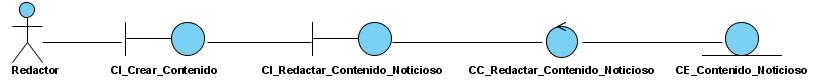
\includegraphics[width=16.5cm,height=1.8cm]{img/DCA_1}}\\
\hline
[Ver diagrama de colaboración asociado \ref{dia: dcarcn}]\\
\hline
\end{tabular}
\caption{Diagrama de clases del análisis - CU Redactar Contenido Noticioso }
\end{figure}



%TABLA VIEW_VIEW
\begin{center}
\begin{longtable}{|p{5.1cm}|p{3cm}|p{8.3cm}|}
%%para pnerle en el pie de la tabla que continua en la otra página
\multicolumn{3}{|r|}{{Continúa en la próxima página}} \\ \hline
\endfoot
% \hline
\endlastfoot

\hline

 \multicolumn{3}{|>{\columncolor[gray]{.9}}l|}{{\bf Nombre:} view\_view } \\ \hline

 \multicolumn{3}{|l|}{ {\bf Descripción:} Información básica de una vista.} \\ \hline

 nodes\_per\_block &  smallint &  Se indica el número de nodos que aparecen en cada bloque. \\ \hline

 menu\_tab\_weight &  smallint &  Se puede indicar el peso de las pestañas para ordenarlas. \\ \hline

 menu\_tab &  smallint &  Se muestra un menú de pestañas. \\ \hline

 menu &  smallint &  Se configuran las opciones para que la vista aparezca en el menú. \\ \hline

 nodes\_per\_page  &  smallint &  Cantidad de nodos por páginas. \\ \hline

 changed &  int &  Fecha en que es modificada la vista. \\ \hline

 vid &  int &  Identificador de la tabla vista. \\ \hline

 block\_footer &  long varchar &  Se indica el pie de página que tendrá la vista. \\ \hline

 block\_header &  long varchar &  Se indica el encabezado que tendrá la vista. \\ \hline

 page\_footer  &  long varchar &  Se indica el pie de página que tendrá la página de la vista en caso de que se muestre en una página. \\ \hline

  page\_empty  &  long varchar &  Indica el texto que se muestra cuando no se
encuentra ningún resultado. \\ \hline

 page\_header &  long varchar &  Se indica el encabezado que tendrá la página de la vista en caso de que se muestre en una página.\\ \hline

 block\_title & varchar &  Se cambia el título de los bloques.\\ \hline

 menu\_title & varchar &  Se indica el nombre título para el menú.\\ \hline

 url &  varchar &  En esta opción tenemos que indicar la url se quiere que tenga la vista.\\ \hline

 access &  varchar & Se indican que roles pueden consultar la vista.\\ \hline

 description &  varchar &  Se describe la vista brevemente.\\ \hline

 name &  varchar &  Indica el nombre de la vista que se va a crear.\\ \hline
\caption{Descripción de la tabla \textbf{view\_view}}
\end{longtable}
\end{center}


\end{document}
